\documentclass[a4paper,12pt,twoside,final,spanish]{article}
%titlepage: pone el título en una página aparte
%twocolumn
\usepackage{babel} %Para el lenguaje [spanish]
\usepackage[utf8]{inputenc} %Para reconocer todos los símbolos
\usepackage[T1]{fontenc}
\usepackage{textcomp}
\usepackage{amsmath}
\usepackage{amsfonts}
\usepackage{amssymb}
\usepackage[margin=2.5cm]{geometry} %Márgenes
\usepackage[T1]{fontenc}
\usepackage{graphicx}
\usepackage{hyperref}
\usepackage{listings} %Para escribir códigos
\usepackage{xcolor}
%\pagestyle{headings}

\lstset { 
  language=Matlab,
  basicstyle=\footnotesize,
  numbers=left,
  numberstyle=\tiny\color{red},
  stepnumber=1,
  numbersep=8pt,
  backgroundcolor=\color{white},
  showspaces=false,               % show spaces adding particular underscores
  showstringspaces=false,         % underline spaces within strings
  frame=lines,                   % adds a frame around the code
  rulecolor=\color{red},
  tabsize=4,                      
  captionpos=b,                   % sets the caption-position to bottom
  breaklines=true,                % sets automatic line breaking
  keywordstyle=\color{blue},          % keyword style
  commentstyle=\color{green},       % comment style
  stringstyle=\color{magenta},         % string literal style
}

\title{\Huge Mecánica Computacional\\
Trabajo Práctico Nº1\\
Introducción y nociones generales}
\author{Darién Julián Ramírez}
\date{\today}

\begin{document}

\maketitle %Crea la página de título

\section{Ejercicio 1}

La figura muestra una micrografía de un espécimen de acero inoxidable aumentado 560 veces. El espécimen fue pulido y atacado químicamente, para poner de relieve su estructura. Se ve que es claramente no uniforme. Sin embargo, si usamos acero inoxidable para construir una caldera, podemos considerarlo como un material homogéneo.

¿Puede justificar esta hipótesis? 

\dotfill

\begin{quote}
Alto de la placa: $h=8.1[cm]$\\
Ancho de la placa: $a=5.8[cm]$\\
Espesor de la caldera: $e=2.54[cm]$\\
Aumento: $560 [veces]$

Se ve que la placa posee imperfecciones para ello hay que determinar un tamaño de imperfección. Entre los valores $h$ y $a$ de la placa, el más representativo es el más pequeño ($a$).

Tamaño de la imperfección: $l=\frac{a}{560 [veces]}=0.010357142 [cm]=1.0357142~\times~10^{-2}~[cm]$

Proporción: $\frac{l}{e}=4.07\times10^{-3}$

Esto quiere decir que el espesor de la caldera es \textbf{mil} veces mayor que el tamaño de la imperfección. Como regla general basta con que la proporción sea \textbf{cien} veces mayor para considerar al material homogéneo.

De este modo el acero inoxidable puede ser considerado un material homogéneo para la construcción de la caldera. 
\end{quote}

\section{Ejercicio 2}

La molécula de agua está hecha de un átomo de oxígeno y dos de hidrógeno. El átomo de oxígeno es más grande que el átomo de hidrógeno. La distancia entre el centro del átomo de oxígeno y el centro del átomo de hidrógeno es de $0,957[A]$ ($1[A]=10^{-8}[cm]$). Las líneas que unen el centro del átomo de oxígeno a los centros de los átomos de hidrógeno forman un ángulo de $105,3º$.

¿Cuál debe ser el tamaño mínimo de un cuerpo de agua para que su movimiento pueda tratarse por métodos de mecánica del continuo? 

\dotfill

\begin{quote}
Lo primero que se debe hacer es determinar cuál es la longitud representativa de la molécula de agua. Se tienen dos posibilidades, la distancia entre el átomo de oxígeno y el átomo de hidrógeno ($OH$) o la distancia entre los átomos de hidrógeno ($HH$).

Distancia entre el átomo de oxígeno y el átomo de hidrógeno: $OH = 0.957 [A]=0.957\times 10^{-8}[cm]$

Ángulo entre las líneas $OH$: $\theta=105.3[grados]$

Para determinar la distancia $HH$ entre los átomos de hidrógeno hay que usar trigonometría:

\begin{center}
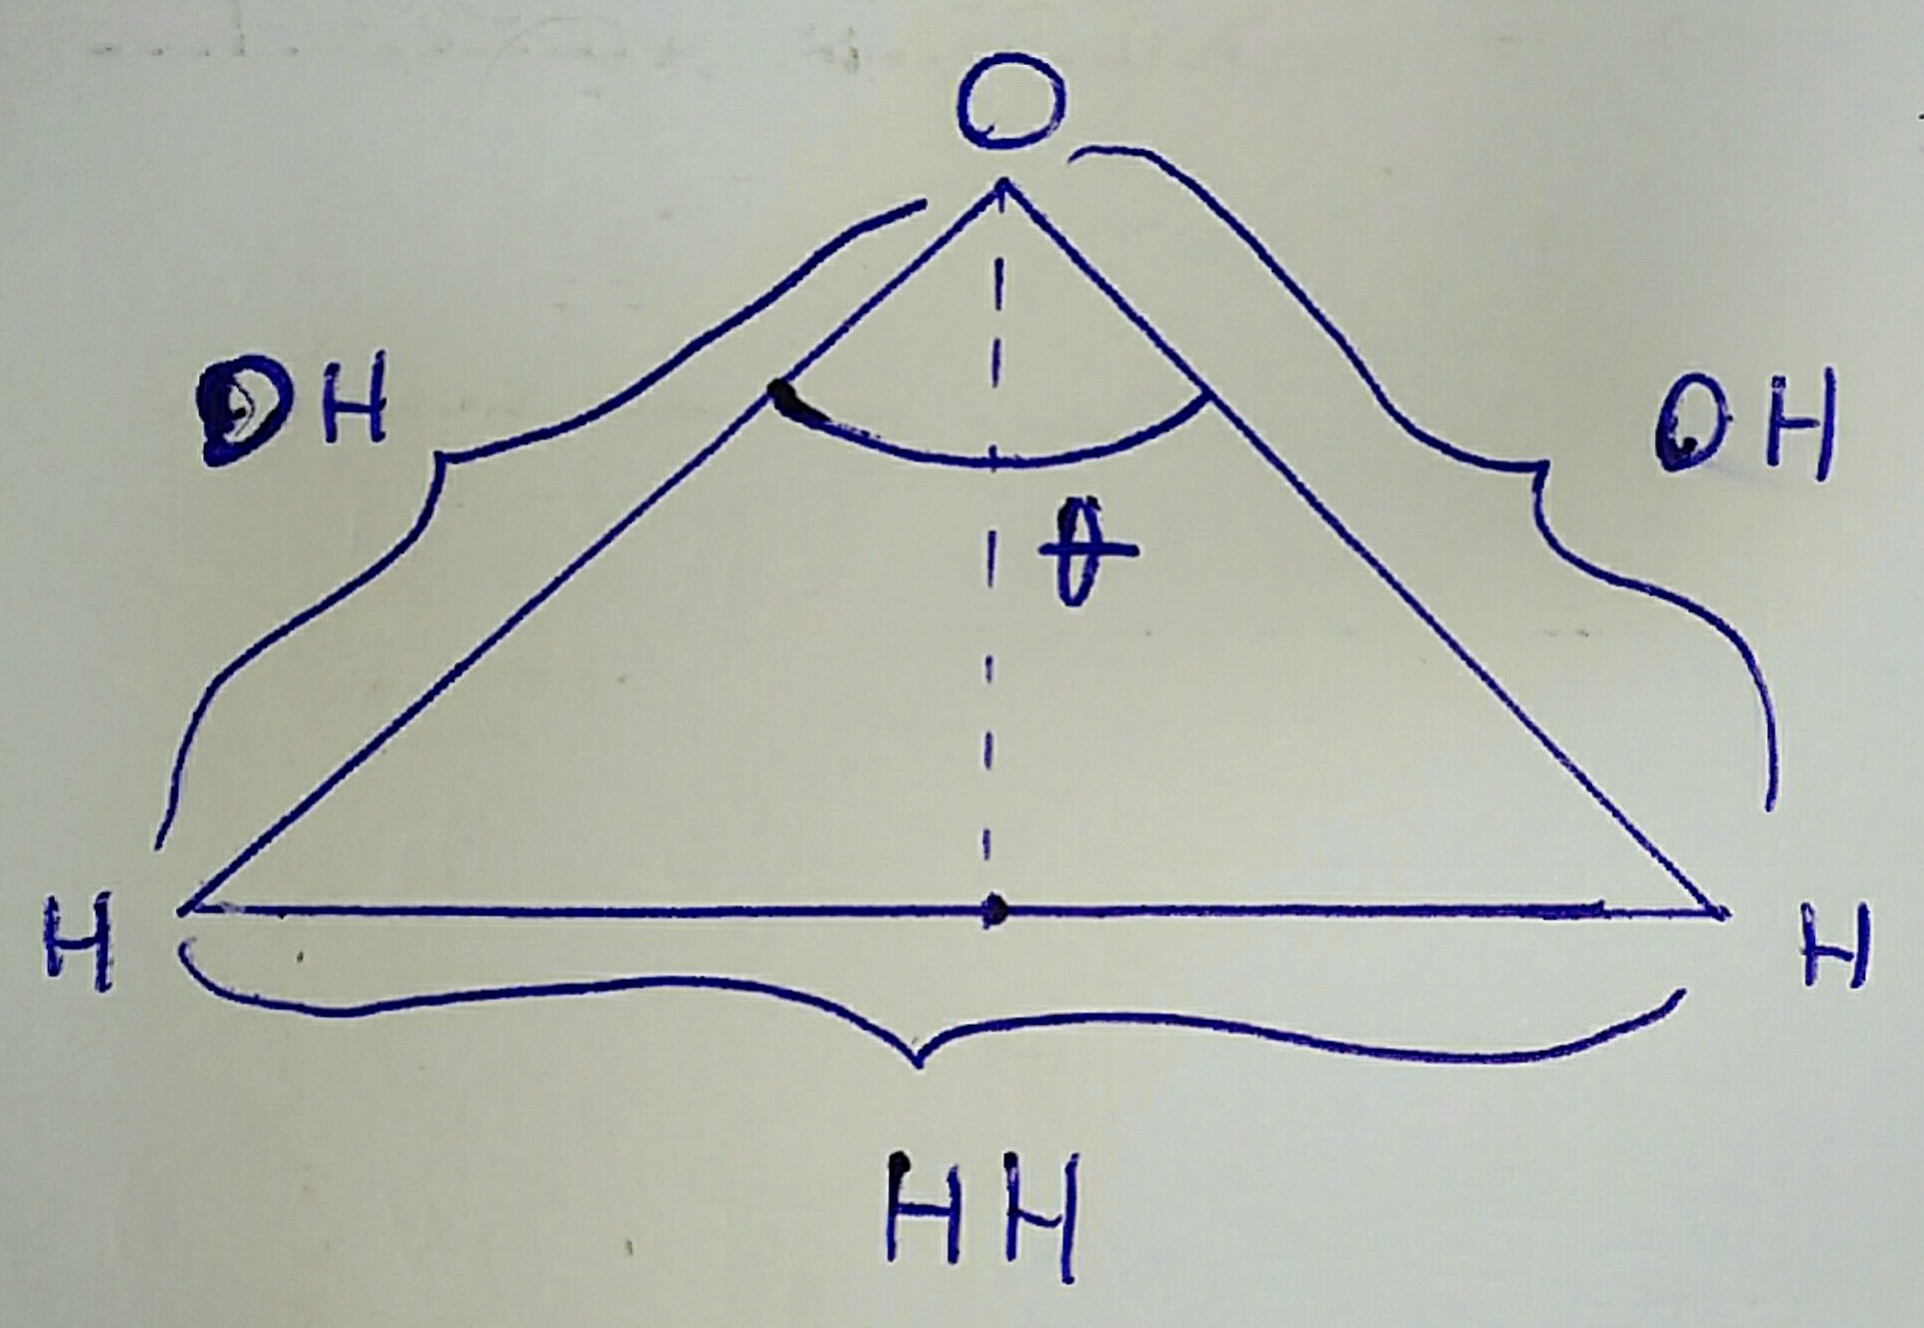
\includegraphics[width=0.5\linewidth,keepaspectratio]{ejercicio2}
\end{center}

$\frac{HH}{2}=OH*\sin{\frac{\theta}{2}} \implies HH=2*OH*\sin{\frac{\theta}{2}}=1.52\times10^{-8}[cm]$

Se puede observar que $HH>OH$ por lo tanto $HH$ será nuestra longitud representativa.

Ahora se sabe que el tamaño de la proporción entre la molécula de agua y el cuerpo de agua debe ser de cien veces o menor:

$\frac{HH}{T}\leq10^{-2} \implies T\geq\frac{HH}{10^{-2}}=1.52\times10^{-6}[cm]$; donde $T$ es el tamaño del cuerpo de agua.

El cuerpo de agua debe tener un tamaño mayor o igual a $1.52\times10^{-6}[cm]$.

\end{quote}

\section{Ejercicio 3}

Para un gas, la longitud del camino libre medio entre colisiones es una medida de la distancia media entre moléculas. Para el aire que se sitúa a un km sobre el nivel del mar, el camino libre medio es $8\times10^{-6}[cm]$; a 100 km de alto se tienen 9,5 cm; a 200 km es de $3\times10^{4}[cm]$. Para analizar el flujo de aire en torno a un cohete reentrando en la atmósfera, ¿sería posible hacerlo por métodos de mecánica del continuo? 

\dotfill

\begin{quote}
Longitud del cohete: $l=100[m]$\\
Diámetro del cohete: $d=10[m]$\\
Camino libre medio a $1[Km]$: $8\times10^{-6}[cm]$\\
Camino libre medio a $100[Km]$: $9.5[cm]$\\
Camino libre medio a $200[Km]$: $3\times10^{4}[cm]$

La longitud representativa en este caso será la menor ($d$).

\begin{itemize}
\item A un kilómetro de altura:

Proporción: $\frac{8\times10^{-6}[cm]*10^{-2}}{d}=8\times10^{-9}$

La longitud representativa del cohete es $10^{9}$ veces mayor que el camino libre medio entre moléculas, por lo tanto el problema puede ser tratado por los métodos de la mecánica del continuo.

\item A 100 kilómetros del altura:

Proporción: $\frac{9.5[cm]*10^{-2}}{d}=9.5\times10^{-3}$

La longitud representativa del cohete es 1000 veces mayor que el camino libre medio entre moléculas, por lo tanto el problema puede ser tratado por los métodos de la mecánica del continuo.

\item A 200 kilómetros de altura:

Proporción: $\frac{3\times10^{4}[cm]*10^{-2}}{d}=3\times10^{1}$

La longitud representativa del cohete no llega a ser 100 veces mayor que el camino libre medio entre moléculas, por lo tanto el problema no puede ser tratado por los métodos de la mecánica del continuo.
\end{itemize}
\end{quote}

\section{Ejercicio 4}

Halle las cargas en las barras a, b, c del reticulado articulado cargado por una fuerza W como se ve en la figura.  


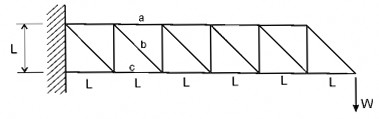
\includegraphics[width=0.9\linewidth,keepaspectratio]{ejercicio4}


\dotfill

\begin{quote}
Supongamos las tres fuerzas $F_{a}$, $F_{b}$ y $F_{c}$ con direcciones arbitrarias como se las muestra en el siguiente diagrama de cuerpo libre:

\begin{center}
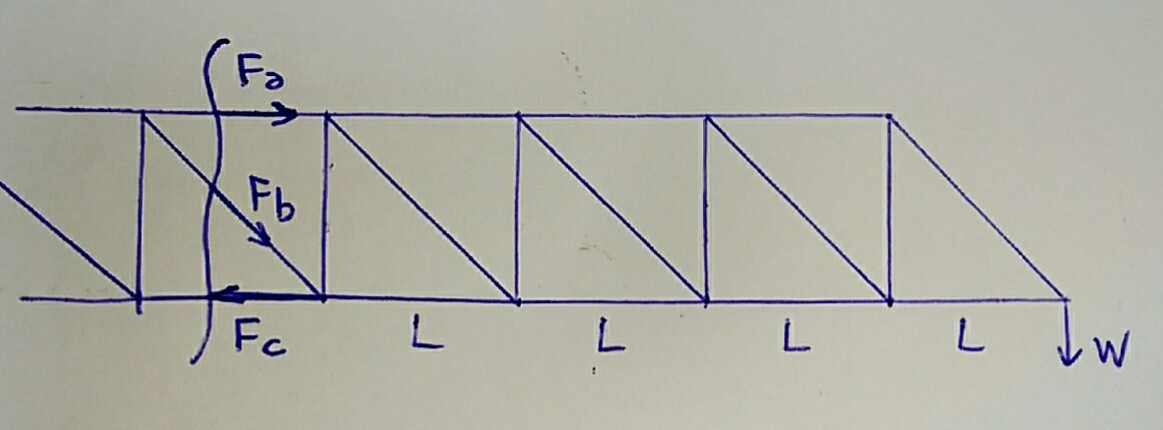
\includegraphics[width=0.8\linewidth,keepaspectratio]{ejercicio42}
\end{center}

Planteamos las sumatorias de fuerzas y momentos con respecto al punto donde convergen $F_{b}$ y $F_{c}$ para simplificar los cálculos:

$\sum F_{x}=F_{a}+F_{b}*\cos(45)-F_{c}=0 \implies F_{c}=-5W$\\
$\sum F_{x}=-F_{b}*\sin(45)-W=0 \implies F_{b}=-\frac{2W}{\sqrt{2}}$\\
$\sum M=-F_{a}*L-W*4L=0 \implies F_{a}=-4W$

Los signos negativos de las fuerzas indican que son en realidad de sentido opuesto. Por lo tanto $F_{a}$ y $F_{b}$ son positivas con respecto a mi sistema de referencia haciéndolas fuerzas de tracción, mientras que $F_{b}$ es negativa con respecto a mi sistema de referencia haciéndola una fuerza de compresión.
\end{quote}

\section{Ejercicio 5}

Un hombre trabaja con una pala en su jardín. Si el peso combinado de la carga y la pala es de 10 kg y su centro de gravedad se ubica a una distancia de 1 metro de la vertebra lumbar en su columna, ¿cuánto será el momento en torno a esa vertebra?

La construcción de la columna vertebral está esquematizada en la figura. Los discos entre las vértebras sirven como pivotes de rotación. Se puede asumir que no resisten momento. Por lo tanto, el peso de la carga y la pala debe ser resistido por la columna vertebral y el músculo. Estime la fuerza que deben realizar el músculo, la vértebra y los discos.

El dolor de espalda es una dolencia habitual. Las cargas realizadas sobre los discos fueron medidas con "strain gauges". Se encontró que la influencia de la presión que se desarrolla en el abdomen por contracción de los músculos abdominales cuando se levanta un peso es importante, y por ello el modelo simplificado del párrafo anterior no es correcto y entrega resultados falsos. En la figura, se muestra un modelo de cuerpo libre de la parte superior del cuerpo de un hombre. Muestre que si se tiene un abdomen grande y músculos abdominales fuertes, disminuyen las cargas sobre el sector de la columna. 

\dotfill

\begin{quote}

\begin{center}
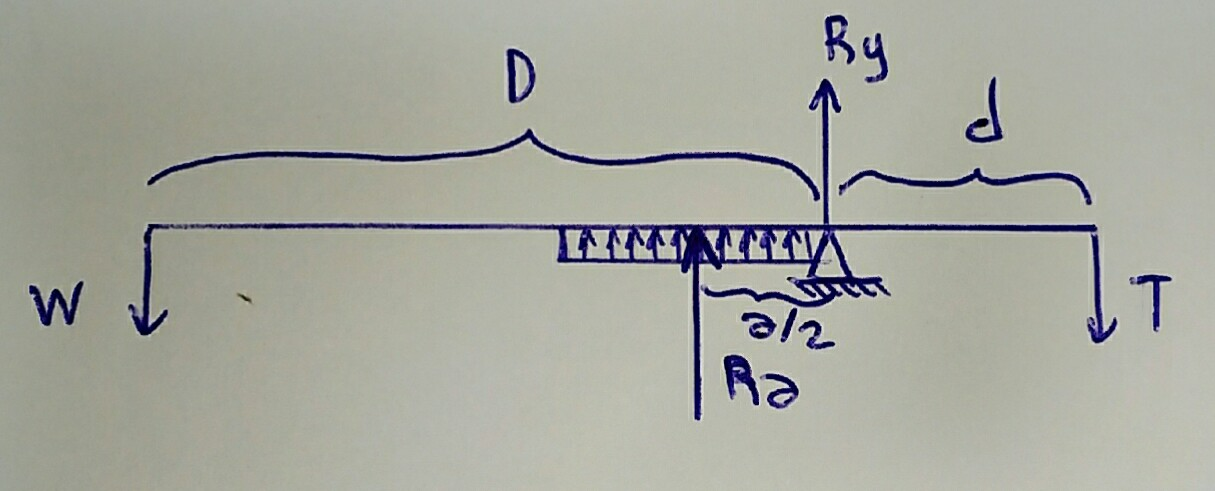
\includegraphics[width=0.9\linewidth,keepaspectratio]{ejercicio5}
\end{center}

$R_{a}=q*a$; q: fuerza distribuida $[\frac{N}{m}]$; a: área $[m^2]$ \\
$\sum F_{x}=0$\\
$\sum F_{x}=-W+R_{a}+R_{y}-T=0 \implies R_{y}=W+T-R_{a}\\ \implies R_{y}=W+\frac{W*D-R_{a}*\frac{a}{2}}{d}-Ra$\\
$\sum M=W*D-R_{a}*\frac{a}{2}-T*d=0 \implies T=\frac{W*D-R_{a}*\frac{a}{2}}{d}$
\end{quote}

\section{Ejercicio 6}

La figura muestra un sistema de 7 partículas en el plano, vinculadas entre sí por resortes, que inicialmente se encuentran en reposo. La masa de las partículas es igual a 0.5, en tanto la rigidez de los resortes es igual a 20 y la longitud L es igual a 5.
\begin{itemize}
\item Desarrolle un programa de computación que calcule la respuesta del sistema a una carga estacionaria W = 5. A partir de los resultados, calcule la fuerza en la 
barra 2-3 y compare con el resultado obtenido siguiendo el método del punto 4.
\item Desarrolle un programa de computación que calcule la respuesta del sistema a la carga dinámica dada en la figura, durante los primeros 50 segundos.
\item Modifique el programa desarrollado, para calcular la respuesta del sistema a una  carga de variación sinusoidal. Experimente calculando la respuesta para excitaciones de diferentes frecuencias. Extraiga conclusiones. 
\end{itemize}

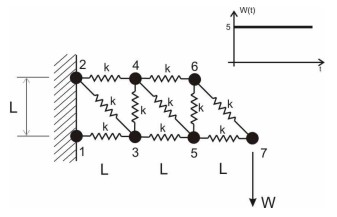
\includegraphics[width=0.9\linewidth,keepaspectratio]{ejercicio6}

\textbf{Sugerencia}: plantear el sistema de ecuaciones diferenciales ordinarias utilizando Matlab y las facilidades de resolución de ecuaciones diferenciales ordinarias disponibles. Presentar resultados en forma gráfica.

\dotfill

\begin{quote}
\begin{lstlisting}
function f = odefunTP1Ej6(t,y)

	% Datos
	
	% Masas de las particulas
	m_1 = m_2 = m_3 = m_4 = m_5 = m_6 = m_7 = 0.5;

	L = 5;

	%Coordenadas iniciales de la particulas
	x0_1 = [0;0];
	x0_2 = [0;L];
	x0_3 = [L;0];
	x0_4 = [L;L];
	x0_5 = [2*L;0];
	x0_6 = [2*L;L];
	x0_7 = [3*L;0];

	% Constantes elasticas de los resortes
	k_13 = k_23 = k_24 = k_34 = k_35 = k_45 = k_46 = k_56 = k_57 = k_67 = 20;

	% Longitudes iniciales de los resortes
	L0_13 = norm(x0_1 - x0_3);
	L0_23 = norm(x0_2 - x0_3);
	L0_24 = norm(x0_2 - x0_4);
	L0_34 = norm(x0_3 - x0_4);
	L0_35 = norm(x0_3 - x0_5);
	L0_45 = norm(x0_4 - x0_5);
	L0_46 = norm(x0_4 - x0_6);
	L0_56 = norm(x0_5 - x0_6);
	L0_57 = norm(x0_5 - x0_7);
	L0_67 = norm(x0_6 - x0_7);

	% Carga
	W = [0;-5];
	
	% Coordenadas actuales de las particulas
	x_1 = x0_1;
	x_2 = x0_2;
	x_3 = y(1:2);
	x_4 = y(3:4);
	x_5 = y(5:6);
	x_6 = y(7:8);
	x_7 = y(9:10);	

	% Longitudes actuales de las particulas
	L_13 = norm(x_1 - x_3);
	L_23 = norm(x_2 - x_3);
	L_24 = norm(x_2 - x_4);
	L_34 = norm(x_3 - x_4);
	L_35 = norm(x_3 - x_5);
	L_45 = norm(x_4 - x_5);
	L_46 = norm(x_4 - x_6);
	L_56 = norm(x_5 - x_6);
	L_57 = norm(x_5 - x_7);
	L_67 = norm(x_6 - x_7);

	% Fuerzas en los resortes
	F_13 = k_13*(1-L0_13/L_13)*(x_3 - x_1);
	F_23 = k_23*(1-L0_23/L_23)*(x_3 - x_2);
	F_24 = k_24*(1-L0_24/L_24)*(x_4 - x_2);
	F_34 = k_34*(1-L0_34/L_34)*(x_4 - x_3);
	F_35 = k_35*(1-L0_35/L_35)*(x_5 - x_3);
	F_45 = k_45*(1-L0_45/L_45)*(x_5 - x_4);
	F_46 = k_46*(1-L0_46/L_46)*(x_6 - x_4);
	F_56 = k_56*(1-L0_56/L_56)*(x_6 - x_5);
	F_57 = k_57*(1-L0_57/L_57)*(x_7 - x_5);
	F_67 = k_67*(1-L0_67/L_67)*(x_7 - x_6);

	% Velocidades actuales de las particulas
	v_3 = y(11:12);
	v_4 = y(13:14);
	v_5 = y(15:16);
	v_6 = y(17:18);
	v_7 = y(19:20);

	f = [
		v_3
		v_4		
		v_5
		v_6
		v_7
		(- F_13 - F_23 + F_34 + F_35) / m_3;
		(- F_24 - F_34 + F_45 + F_46) / m_4;
		(- F_35 - F_45 + F_56 + F_57) / m_5;
		(- F_56 - F_46 + F_67) / m_6;
		(- F_57 - F_67 + W) / m_7;
		];
end
\end{lstlisting}
\begin{lstlisting}
L = 5;
tfinal = 1;

y_0 = [L 0 L L 2*L 0 2*L L 3*L 0 zeros(1,10)];

[tout, yout] = ode23s(@odefunTP1Ej6,[0 tfinal],y_0);
\end{lstlisting}
\end{quote}

\begin{thebibliography}{1}
\bibitem{MCF}
Y. C. Fung,
\emph{A First Course in Continuum Mechanics}, 
tercera edición,
PRENTICE HALL,
1994.
\end{thebibliography}

\end{document}